%-----------------------------------------------------------------------------------------------------------------%
\documentclass[10pt,compress,xcolor=dvipsnames]{beamer}    %For presentation version

%% ----- Theme for projector display version --------------
\mode<presentation> {
      \definecolor{Verde}{RGB}{05,130,25}
    \usecolortheme[named=Verde]{structure}
    \useinnertheme{rounded} %%rectangles, circles, rounded, inmargin,
    \useoutertheme{split} %%puts sections on the upper-left hand side and subsections in upper-rhs; name and title on the lower (watch out for page nums)
\setbeamertemplate{navigation symbols}{}  %%Get rid of the navigation symbols at the bottom
}  %%END OF MODE PRESENTATION

%% -------------- Packages ------------------------------ %%
%\pdfoptionpdfminorversion=6 %some attachments are PDF version 1.6 and I get an error
\usepackage[english]{babel}

\usepackage{amsfonts}
\usepackage{amsmath}
\usepackage{amssymb}
\usepackage{amsthm}
\usepackage{mathtools}
\usepackage{graphicx}
\graphicspath{{./include/}}% where figures are saved  %%must \usepackage{graphicx}
\usepackage{comment,footmisc,pdflscape,array,booktabs}
\usepackage{lmodern}  %%allowing font sizes at arbitrary sizes // removes LaTeX Font Warning: Font shape `OT1/cmss/m/n' in size <4> not

\usepackage{hyperref}
\hypersetup{
   colorlinks = true,
   citecolor = {Verde},
   linkcolor = {Verde},
   menucolor = {Verde},
   filecolor = {Verde},
 }
























%%%%%%%%%%%%%%%%%%%%%%%%%%%%%%%%%%% TITLE %%%%%%%%%%%%%%%%%%%%%%%%%%%
%\title[GxInsurance]{\textbf{Moral Hazard Heterogeneity: Genes, Health Insurance, and Smoking Decisions after a Health Shock}}
%\author[Pietro, Laura]{Pietro Biroli and Laura Zwyssig}
%\institute[UZH]{University of Z\"urich}
%\date{\color{red} EALE-SOLE-ASSLE World Conference \\ \color{blue}{June 25, 2020}}
%


\begin{document}
%
%\maketitle
%
%%------------------------------------------------------------------------%
%%% INTRODUCTION %
%%------------------------------------------------------------------------%
\section{Research Question}
%--------------------------------------------------------------%
\begin{frame}
\frametitle{Moral Hazard Heterogeneity: Genes, Health Insurance, and Smoking Decisions after a Health Shock}
\framesubtitle{\hspace{33ex} \textit{by Pietro Biroli and Laura Zwyssig}}

%%%What is the question I want to answer?
\textbf{What}:
	\begin{itemize}
		\item Does reaction to a negative health shock depend on health insurance and genetic differences?
	\end{itemize}

  \vspace{2ex}
 % \pause

%%%How do I answer the question
\textbf{How}:
\begin{itemize}
  \item Focus on smoking behavior following a cardio-vascular health shock
  \item Identification: US adults who receive free health insurance coverage after 65 (Medicare) (see Marti and Richards, 2017)
  \item Compare high and low genetic predisposition to smoking (G$\times$E)
\end{itemize}

  \vspace{2ex}
%  \pause

%%%Why do we care?
\textbf{Why}:
\begin{itemize}
		\item Interplay between financial and biological constraints:
		\begin{itemize}
			\item Health insurance buffers financial consequences of health shocks
			\item Genetic predispositions influence behavioral responses
		\end{itemize}
			\item Understand who is at the margin
		\item Individualized health insurance profiles?
\end{itemize}
\end{frame}



%--------------------------------------------------------------%
\section{Regression}
%--------------------------------------------------------------%
\begin{frame}
\frametitle{Regression results}

\hspace{-5ex}
\begin{minipage}{.49\textwidth}
	\begin{table}[ht]
		\caption{Effect of the health shock} %by timing and PGS
		\small\resizebox{0.65\textheight}{!}{
		% latex table generated in R 4.0.2 by xtable 1.8-4 package
% 
\begin{tabular}{lll}
  \toprule
  \multicolumn{3}{c}{ \textbf{Effect of health shock on smoking probability}} \\
 \midrule
 & Low PGS & High PGS \\ 
   \midrule
Pre 65 & -0.165** & -0.108 \\ 
   & (0.069) & (0.083) \\ 
  Post 65 & 0.09*** & -0.13 \\ 
   & (0.026) & (0.089) \\ 
   \toprule \multicolumn{3}{c}{ \textbf{Effect of health insurance on effect of health shock}} \\
 \midrule
 & Low PGS & High PGS \\ 
   \midrule
Post 65 - Pre 65 & 0.256*** & -0.023 \\ 
   & (0.079) & (0.121) \\ 
   \toprule \multicolumn{3}{c}{ \textbf{Differential effect of health insurance by genetic group}} \\
 \midrule
 & High PGS  & - low PGS \\ 
   \midrule
Post 65 - Pre 65 & -0.279* &  \\ 
   & (0.144) &  \\ 
   \bottomrule
\end{tabular}

		}

		\vspace{1ex}

		{\raggedright \tiny \textit{Notes:} Summary of the effect of the shock on smoking for those who were uninsured before 65, stratified by timing of the shock (before vs. after 65) and genetic group (high vs. low PGS) \par}
	\end{table}
\end{minipage}
%
\hspace{4ex}
%
\begin{minipage}{.49\textwidth}
	\vspace{5ex}
	\begin{figure}[hbtp]
	\centering
	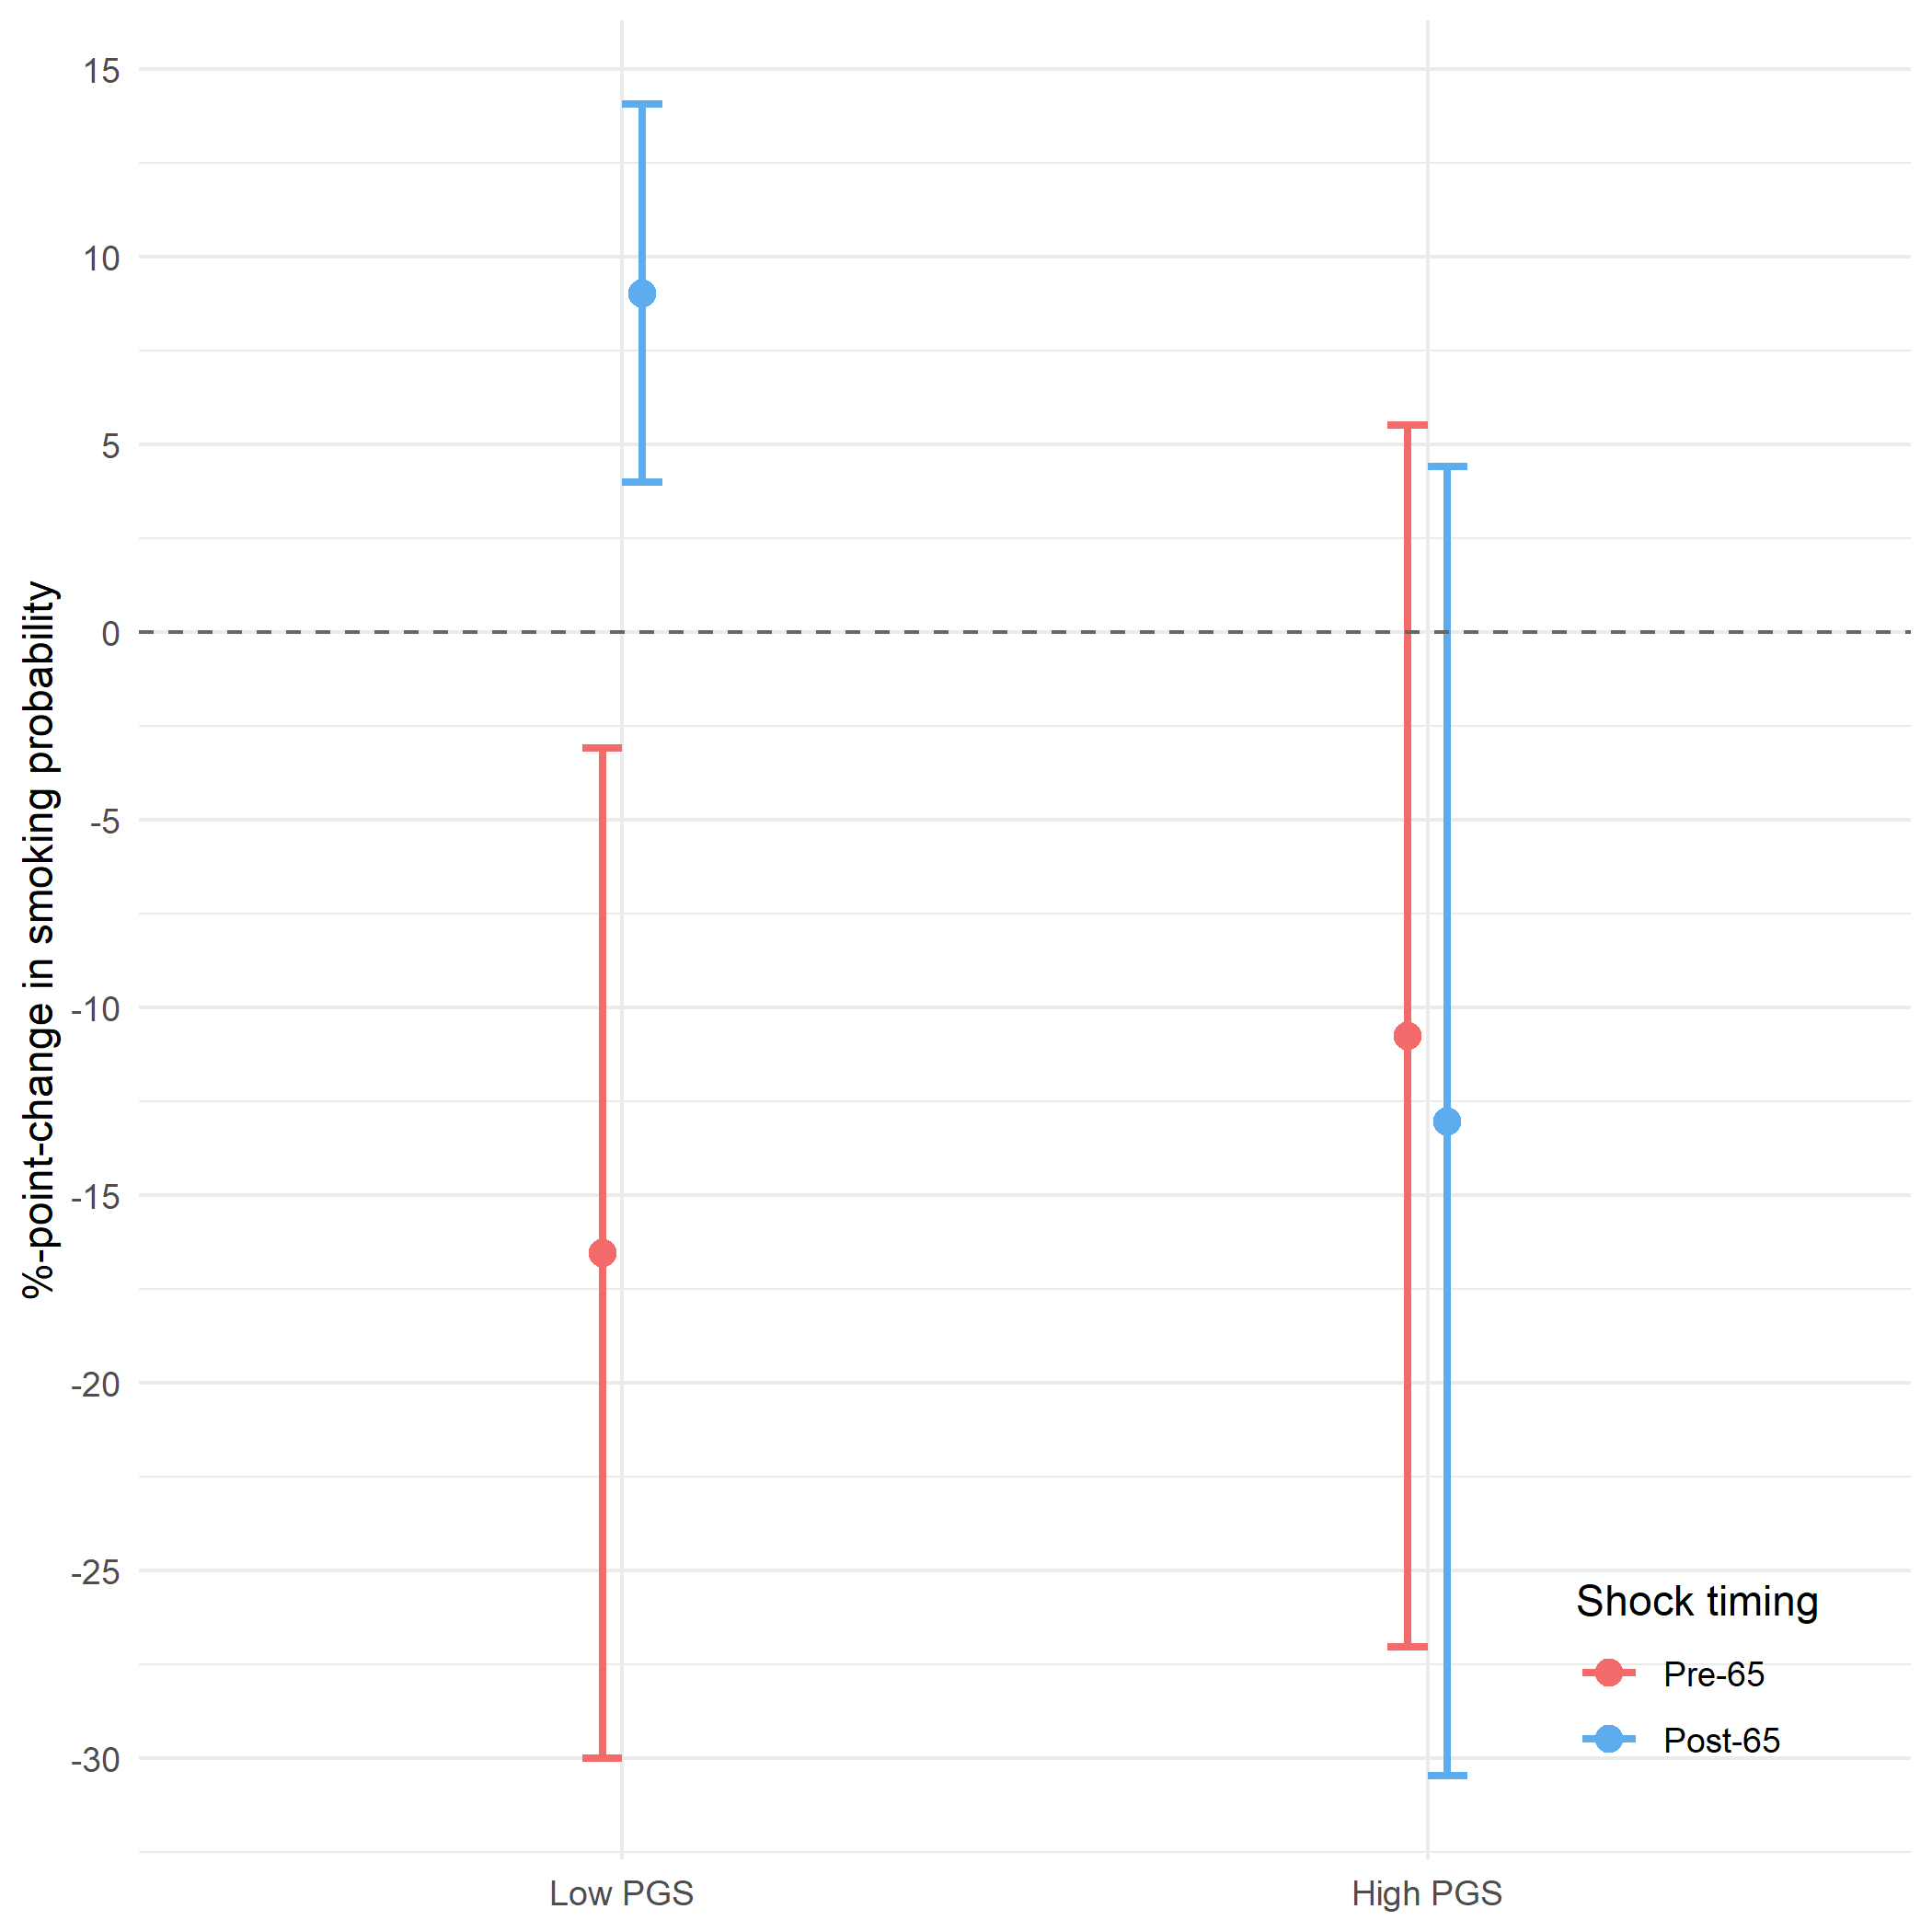
\includegraphics[height=0.65\textheight]{../../3_output/shock_effects/main_6070_100_cvplot.png}
	\label{fig:maincoeffplot}
	\end{figure}
\end{minipage}

\end{frame}


%--------------------------------------------------------------%
\section{Conclusion}
%--------------------------------------------------------------%

%--------------------------------------------------------------%
\begin{frame} \frametitle{Conclusion}
\begin{itemize}
	\item Results:
	\begin{itemize}
		\item Health shock when uninsured $\Rightarrow$ less smoking...
		\item ... but \textit{only} for low PGS.
		\item Effect size is quite sizable (36.7 pp)
	\end{itemize}

	\vspace{3ex}

	\item Interaction between financial and ``biological'' constraints:
	\begin{itemize}
		\item Health insurance buffers financial consequences of health shocks
		\item Genetic predisposition to smoking mutes this effect (lower elasticity)
	\end{itemize}

	\item[$\Rightarrow$] Environment \emph{and} genes jointly influence healthy behaviors

	\vspace{3ex}

	\item Biological foundation of heterogeneity in \textbf{moral hazard} (Einav et al. 2013) %\cite{Einav2013}
	\item[$\Rightarrow$] Biological predispositions can tell a story about choices and economic fundamentals

\end{itemize}
\end{frame}

\end{document}
